\section{Theory}
\label{sec:theory}

\newtheorem{prop}{Proposition}[section]

%Here we investigate the correctness and expressiveness properties of \sysname. We are mainly concerned with answering the following questions: (1) does the distributed, compiled policy faithfully implement the user's policy regardless of failures? (2) Are the resulting BGP configurations stable?, and (3) what polcies are or are not expressible in \sysname?

If \sysname compiles a user policy to a distributed implementation, then that distributed implementation faithfully meets the centralized policy's semantics under any failure scenario. We are primarily concerned with the steady state: that is, what happens after (if) the routing protocol converges.  We argue that \sysname is correct by breaking down the claim into two distinct parts:

\begin{prop}
A distributed BGP configuration is \textit{Sound} with respect to a \sysname policy, if the any route traffic takes in the network, is a valid route specified in the policy.
\end{prop}

The Soundness claim follows directly from compilation of the product graph. Since every path through the product graph (from start to end) must match the user's policy, and since the compiled configurations use communities to ensure only valid routes through the product graph are used, the resulting BGP configurations are Sound. 

\begin{prop}
A distributed BGP configuration is \textit{Complete} with respect to a \sysname policy, if the distributed implementation always obtains a most preferred route between two nodes when the corresponding path exists in the network.
\end{prop}

%The argument for completeness is as follows: Assume the most preferred path that exists in the network is between two nodes $X$ and $Y$.  This means there is a valid path in the product graph corresponding to this path, and which is available in the network. 
%Assume we are unable to achieve this route in the network. To not achieve this path means that some router along the advertisement route from $Y$ to $X$ preferred to accept an advertisement from another peer instead. This implies that router that makes the ``wrong'' choice appears as a separate node in the product graph. However, from our failure safety check, we know that the other, more-preferred node must have a superset of the paths to accepting states as the less preferred node (from which it stole the route) for at least as good of a final preference. The argument then proceeds by induction on the path length - there are only a finite number of such stealings that can occur, each of which will ultimately still result in a route advertisement reaching $X$ along a most preferred path.

Any \sysname-compiled policy will be \textit{Complete} as a result of the failure safety check.
%
The combination of Soundness and Completeness ensures that the distributed implementation will always achieve the best routes possible, yet will never also use any unwanted routes. 

\begin{prop}
The internal routers in a distributed BGP configuration produced by \sysname will be stable. 
\end{prop}

The reduction is via the well-known No-Dispute-Wheel condition~\ref{bib:todo} for stable BGP. In particular, any policy with a dispute wheel will not pass the stronger failure safety check by \sysname.

%\begin{figure}[t!]
%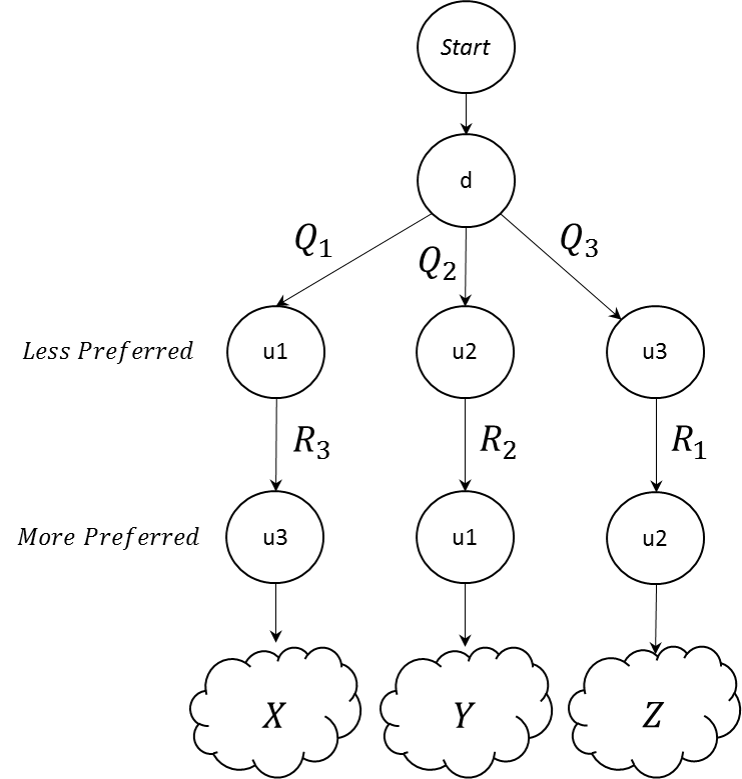
\includegraphics[width=\columnwidth]{figures/dispute-wheel}
%\label{fig:dispute-wheel}
%\caption{Product graph for a dispute wheel.}
%\end{figure}

%The reduction is via the well-known No-Dispute-Wheel condition~\ref{bib:todo}. If a set of BGP configurations do not have a dispute wheel, then they will converge to their best routes. Any BGP policy with a dispute wheel will not satisfy the failure safety condition in Section~\ref{sec:compilation}. Assume that the preferences in the policy describe a dispute wheel, and we will show that our failure check will reject the policy. Informally, a dispute wheel occurs when there are some number of nodes $u_1, \dots, u_n$ attempting to get a path to a destination node $d$. Each node $u_i$ prefers to go through its neighbor $u_{i+1}$ over route $R_i$ than directly to $d$ with route $Q_i$. Thus the nodes form a wheel of preferences. The product graph for a policy that contains a dispute wheel will look like Figure~\ref{fig:dispute-wheel}, which shows a dispute wheel of size 3. In order to pass the failure safety check for the compiler, the more-preferred node for $u_2$ will need to have a superset of the paths starting from the less-preferred node for $u_2$. In turn, this means that the maximum length path after visiting the more preferred $u_2$ will be $max(Z) = 1 + max(Y)$, similarly, if we look at $u_1$, we will determine that $max(Y) = 1 + max(X)$, and so on. The resulting equations define a system of unsatisfiable equations. Therefore, it is not possible for \sysname to compile a BGP policy that contains a dispute wheel. Since no-dispute-wheel is a sufficient condition for BGP stability, any compiled \sysname policy will be stable.

An important distinction is that BGP might still be instable with respect to other external ASes, since \sysname has no way of configuring their routing policy and can only rely on AS path filters to see what advertisements are observed.
